\section{Rotating/Twisting Bezier Splines}

    \subsection{Introduction}
    The first part of the main problem is extracting digital machine data from the existing calligraphy specimens.  Conventionally, image processing is being used [cite?] to extract data that can be used to create machine data. We, however, propose a difference; no matter how strong and robust image processing gets, we propose that there is no alternative to the minor details only a real artist can observe and recreate. So a solution is needed that fulfils the technical needs as well as the artistic demands.

    \subsection{The Necessity}
    One potential way to solve the modeling issue of calligraphy involves using the existing digital calligraphy fonts. There are, however, two critical issues involved with this scheme; one is the need of an algorithm that will convert the font data to robot movement data and the other is the lack of a font variety. Additionally, working with fonts leaves a narrow space of modifying the scripts to look like artistic scriptures. This is the primary reason we must not use the existing digital fonts.
    
    Keeping in mind the gaps left by the digital font, another solution to this problem is in the discovery of a new way to unify ink-mark information of digital Islamic script and tool movement performed by the artist. Making a mathematical model to learn the drawing tool information just from the printed text is quite a complex job. Instead, only if we could form a way an artist can give digital input, this problem can be overcome.

    This is where the twisting Bezier splines come into play. We add a twist/rotation handle in the conventional Bezier spline curves and that is it. The, however, remains unanswered, what is a Bezier spline curve in the first place.

    \subsection{Mathematical Model of a Rotating Bezier Spline}
    \subsubsection{The Conventional Bezier Spline}
        In order to describe how twisting splines work, lets first look into the working principle of a conventional Bezier spline. Figure 1 shows an illustration of a spline path made up of several sub curves. Each curve section is only partly independent of the other. Figure \ref{Fig:RotatingBezierSplines}  (a) shows the final shape of the curve without any construction elements. In Figure \ref{Fig:RotatingBezierSplines} (b), we explode different sections of the curve into smaller elements and show how they fit together to form the complete spline. There five sections in this curve labeled $1$ through $5$. Figure \ref{Fig:RotatingBezierSplines} (c) shows an assembled form of these five sections. It also shows, what are called, anchors and construction handles. The anchor is the point that sits at the terminals of two adjacent curve sections. For instance, Anchor point $A$  is connecting the sections $1$ and $2$. Like all the other anchors, this angle also has two handles, $H_1$ and $H_2$, connected through a straight line passing through the anchor. The length of each handles, $\overline{AH_1}$  and $\overline{AH_2}$ on both sides of the anchor define the shape of the curve section on their respective side where as the orientation of line connecting both handles contributes to the shape on both the curve sections. This is how both section become partly independent. For instance, handle $\overline{AH_1}$ contributes to the shape of curve segment $1$ and $\overline{AH_1}$ to section $2$.


        \begin{figure}
          \centering
          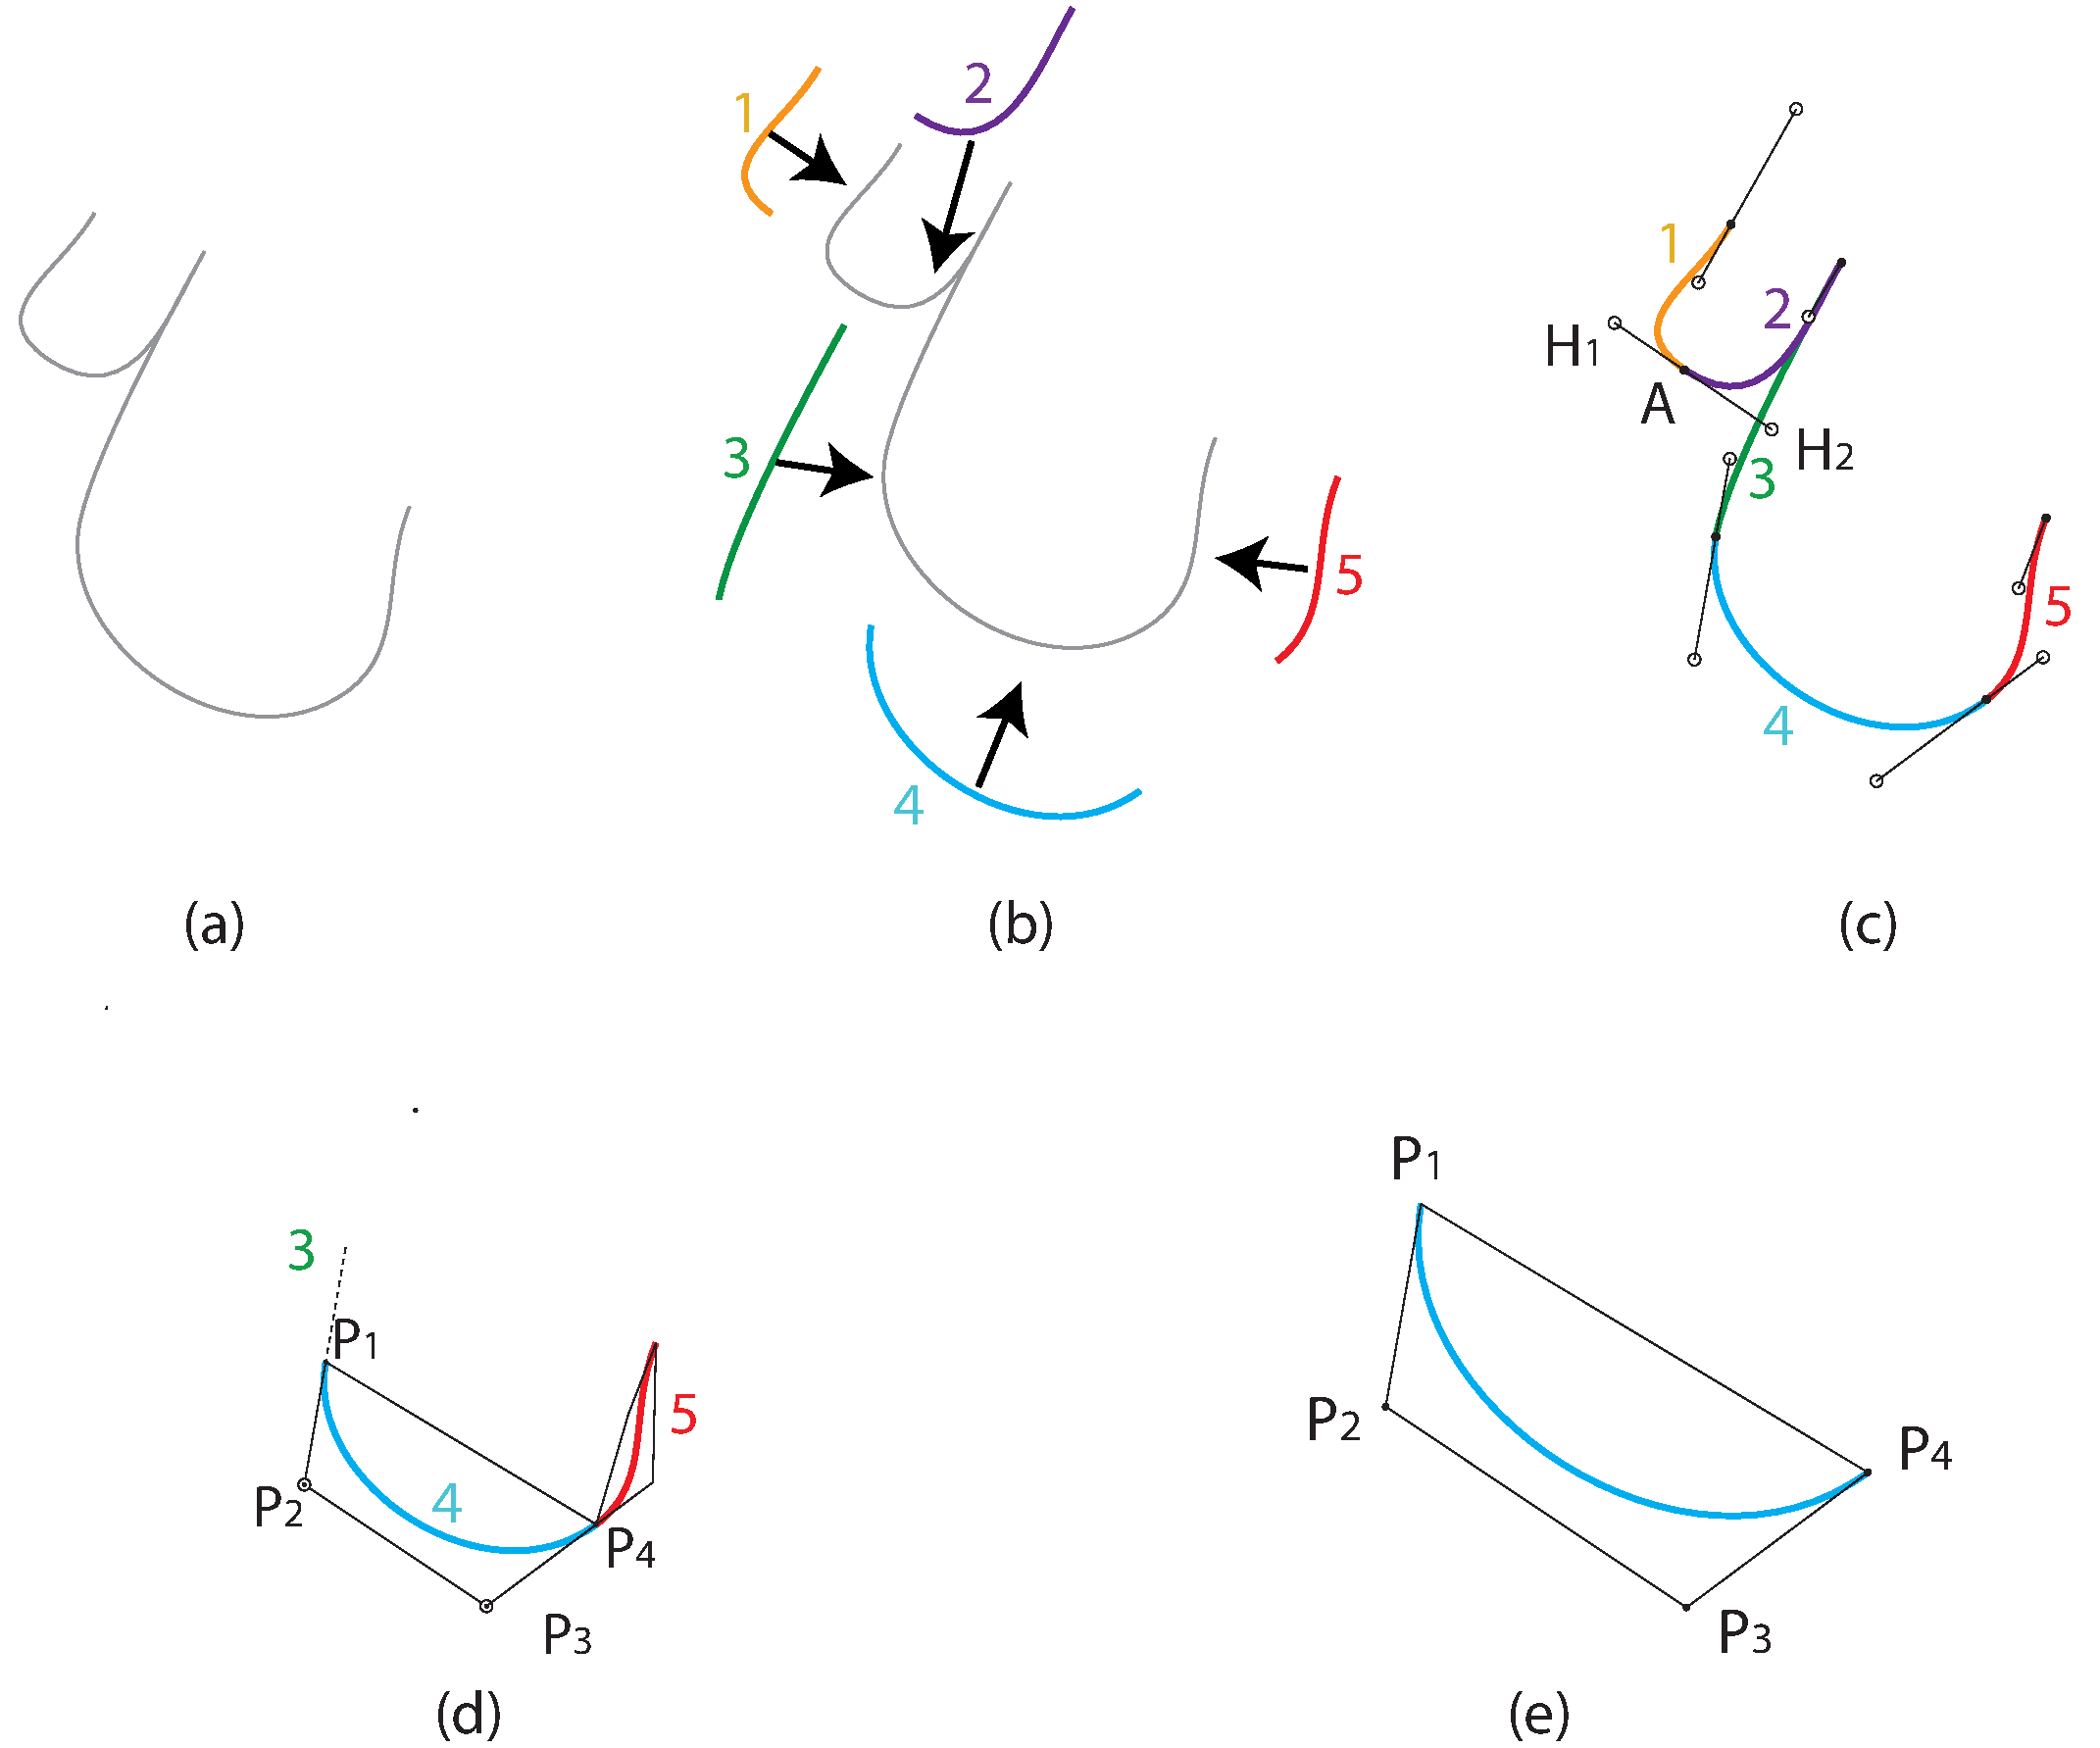
\includegraphics[width=0.9\textwidth]{BezierSplineCurve.pdf}
          \caption{An illustration showing the construction of Bezier Spline Curve. (a) A sample of a Bezier spline path (b) an exploded view of inner curves of the Bezier spline path (c) Handles that control the shape of the two adjacent sub curves (d) and (e) Construction polygon of the sub curve.
          } \label{Fig:RotatingBezierSplines}
        \end{figure}

        Now, it may look like the shapes defined in this way are pretty organic but in fact, the whole shape is defined by simple mathematical equations. Figure \ref{Fig:RotatingBezierSplines} (d) focuses on section $4$ and $5$ of the curve and also shows a polygon defined by the points $P_1$, $P_2$, $P_3$ and  $P_4$. It must be noted that the points $P_1$ and $P_4$ of this polygon are also the anchor point between sections $3$, $4$ and $5$. Take section $4$ for example here. The polygon mathematically defines the complete shape of this polygon. If $P_spline$ is point on the section $4$, with coordinates $x$ and $y$ in a cartesian plane with some origin, it is defined by the following equation.
         \begin{equation}
         P_spline$$=$$P_b×f+P_a×(1 -f)
         \end{equation}
where,
\begin{equation}
P_a=P_23×f+P_12×(1 -f)
\end{equation}
and
\begin{equation}
P_b=P_34×f+P_23×(1 -f)
\end{equation}
where,
\begin{equation}
P_12=P_2×f+P_1×(1 -f)
P_23=P_3×f+P_2×(1 -f)
\end{equation}
and
\begin{equation}
P_34=P_4×f+P_3×(1 -f)
\end{equation}
for an $f$ in the range $[0, 1]$.

It can also be proved that the side segments of the polygon $\overline{P_1 P_2}$ and $\overline{P_3 P_4}$ are tangent to the curve at the point the meet it at $P_1$ and $P_4$ respectively.


\subsubsection{Twist/Rotation Handle}
    On top of the conventional Bezier splines, that work around anchor points that have curvature handles, we add a “Rotation”/”Twist” handle in the anchor and a thickness parameter to the whole curve. A rotation handle is like the curvature handle discussed earlier, except it does not have any effect on the shape of the curve. The thickness parameter defines the size of a flat line centered on $P_spline$ and sweeping on it. The orientation of this sweeping line is the same as the angle between the twist handle and the respective anchor. See Figure 2 (a) that shows rotation handles added in the example under discussion. It must be noted that the curvature of the spline remains the same after adding twist handles that are lying horizontally yet. We then add thickness to the curve in Figure 2 (b). The resulting curve may look a little out of order but it is normal. This is because the rotation handles are lying on their default position. The twist handles may be given some length but it is insignificant since the twist of the curve will only take the value of the angle the handle subtends about the anchor.

    In simpler words, it’s similar to sweeping a pen centered on the actual spline while twisting it uniformly and continuously about its own axis according to the equation
    \begin{equation}
    \theta_twist$$=$$\theta_A  (1-f)+ \theta_B
    \end{equation}
    where $f$ is the same factor that was used to define $P_spline$ and $\theta_A$ and $\theta_B$ are the angles between the first and the second anchor and their rotation handles respectively. It may be noted that since each anchor is connecting two adjacent sub curves, the ending angle of the sweeping line at the end of the first curve is always the same at the beginning of the later. This visually hides the transition of the twisting curve from one sub curve to the other.

    It must also be noted that the angle of rotation handle cannot be constrained in a $2\pi$ domain. Instead, it is completely unbounded, and the sweeping pen may actually take multiple turns both clockwise and anticlockwise while moving on a single curve section as well as the whole curve. When the idea of the twisting splines was first conceived, it wasn’t envisaged that the angle had to be taken like in this scheme. Special care had to be taken in order to graphically read a continuous angle from the user.

    See Table 1 in Appendix which compiles the rectangular coordinates of all the anchors of the rotating bezier spline shown in discussed in this example. Also, see code snippet 1 in appendix which shows the contents of a file that can be used to recreate the spline. In chapter 3, we will discuss “Gregor”, the tool that uses this data to save the created splines.

\subsection{Conversion of Existing Calligraphy Artwork}
Instead of using image processing to try to extract data from existing scans and photographs of the artworks, using rotating Bezier splines we can now include the artists in the process. Just like any other computer-based graphics design application, either we can write a rotating Bezier splines curve editor plugin for an existing open-source application like GIMP [14] or Inkscape [15]. Unfortunately, the later is not a suitable option because the support for the plugins and extensions for both of these poplar software only lets the developer work with the image saving and processing, they don’t let us play with the behavior of the workspace which would be needed to convert the conventional spline tool into a rotating Bezier spline editor. It can still be done by modifying the source code and building the applications from the scratch.

With the second option not viable anymore, we are left with only one option. Writing our own tool to create, modify, save, and reload rotating Bezier splines. Like any other application, for it to be called a “Software”, we also develop some comprehensive documentation discussing the working and behavior of the tool. Although we will discuss in detail about the tool in chapter 3, the fundamental problems it must solve are

\begin{itemize}
\item easy to use interface
\item converting the existing photos to digital form and,
\item generating machine data that that encapsulates the pen rotation information along with other positional and speed information.
\end{itemize}

Keeping in view these requirements we created “Gregor”, the first tool to edit, modify and create rotating Bezier splines. It will be discussed in detail in later chapters

\subsection{Machine Data Generation}
The rotating spline curves are themselves an emulated ink-mark of a broad edge marking tool. This is the reason extracting machine data and even G-codes from them becomes natural. If the flat side of the tool is assumed to be entirely touching the writing surface, the minimum information required to draw a stroke trickles down to the line on which the pen must move and the twist of the pen in world coordinates. This is exactly the rotation Bezier splines can contain once an artist has drawn them on the computer screen. In other words, to call the rotation Bezier splines the machine data, the following assumptions must be made:
\begin{itemize}
	\item The flat tip of a broad edge tool is always completely touching the drawing area.
	\item The inclination of the pen with respect to the drawing area or with respect to the direction of the drawing is either normal or always fixed at an angle and is set by the machine.
	\item To produce thinner strokes, another spline will be used. This means that the machine would have to use multiple tools for such splines.
	\item The axial pressure the pen inserts on the drawing board while drawing is also fixed and the is set by the machine.
\end{itemize}

It is now obvious that to remove the limitations of fixed angles and pressure values, one can add more handles similar to the rotation handle. A set of by directional inclination handles can be added right away with a three-dimensional pen position visualizer to assist the artist determine what angle they want to keep the pen at while drawing a specific stroke. The pressure angle, however, would not be recommended without interfacing some hardware that lets artist feel the pen pressure in real time before setting a handle value. This can be done using a pressure sensitive digital pen or writing tablets [16-18].
There is more detail on how the spline data is converted into machine data in the coming chapters.

\subsection{Characterization}
An important aspect of fabricating a new technique is measuring how well it performs in different usage scenarios. The problem is, in terms of arts, not every mistake the technique makes can be regarded as an issue. Developing a metrics for judging the artistic quality of a calligraphy specimen produced by the Bezier or rotating Bezier splines is altogether a separate discussion and out of scope of this project. However, there are some aspects that we have tried to measure that gives us some idea how effective the rotating Bezier splines can be.

\subsection{Supported Scripts}
The mainline scripts are not necessarily as mathematical as the model of the rotating Bezier splines. Especially, if the artists start to utilize their writing tool in unique ways to extract some unique value from the scripts they create, forming a mathematical model becomes practically impossible. However, since it would be an artist who will be creating and tracing scripts on the screen of a computer, it was safe to claim that given the similarity of the emulation, rotating Bezier splines can be used to produce any script that is written with broad edge tools. However, these are some limitations with this statement:

\begin{itemize}
\item If the tool changes thickness during a stroke (like a flexible brush), the best alternate to achieve a similar appearance of the script would be to use multiple splines with multiple thicknesses that overlap each other in a gradual manner.
\item Although the rotating splines have a defined tool width, the still assume the tool to infinitely thin on the other side, more like a narrow line. This makes negligible but still some difference when the virtual tool is replaced with an actual tool. One way to overcome this issue would to come up with another rendering algorithm that also asks for the missing information. This has been discussed in later chapters when we suggest some other improvements in the overall project.
\end{itemize}
With these assumptions in mind, the “Gregor” was coded.
\subsubsection{Coverage}
\begin{tabular}{|c|c|}
  \hline
Metrics & Results \\
  \hline
Percentage of area outside the original bounds & Less than 2 \\
Percentage of area covered&Better than 94 \\
Maximum lateral deviation of the Bezier path from the pitch line & N.A. (This list was planned in the synopsis but is no longer valid given the nature of fabricated splines.) \\
Total number of compatible scripts & Broad edge scripts of all languages \\
  \hline
\end{tabular}

Please note that the third metrics in this list was planned to be used but is no longer valid given the nature of fabricated splines.
There are also some other metrices that were not measured because of lack of resources and because they required testing the tool with a large group of actual artists.
\begin{tabular}{|c|c|}
  \hline
  Metrics & How can it be measured \\
  \hline
Easy of usage & A survey based on Likert scale \\
Time efficiency of tracing an existing specimen. & Comparison of the time taken by the same artists tracing with conventional and rotating Bezier splines \\
The artistic quality of the specimens produces. & A survey based on Likert scale and filled by a wide range of artists \\
\end{tabular}

\subsubsection{Sample Results}
As a test and a tribute, two scripts by the famous teacher, artist and author of 18 calligraphy books, late Khursheed Gohar Qalam of the National College of Arts (NCA) cite ??? were borrowed; one in Nastaleeq and other in Thuluth.

\subsubsection{Performance with Different Scripts} 